\chapter{Versuchsaufbau und -ablauf}\label{Kap3}

Das folgende Kapitel beschreibt Ziele der Messung, Versuchsaufbau und -durchf"uhrung. Anschlie\ss end werden die erzielten Messergebnisse dargestellt. 

\section{Zielsetzung, Aufbau und Art der Messung}\label{Ziel}

Es stellen sich zwei Fragen: Welcher Art ist die Messung und welche Voraussetzungen m"ussen hierf"ur erf"ullt sein? 

Ziel der Untersuchung sind Erkenntnisse "uber das Skalierungsverhalten des Bramble unter der Arbeitslast von HPL und STREAM. Dazu werden wie in Kap. \ref{Kap2} beschrieben zwei Ma\ss zahlen betrachtet: Performance und Energieverbrauch.

Die Benchmarks werden auf $n-4$ RPi-Knoten des Bramble ausgef"uhrt. Maximal 19 RPi-Knoten werden daf"ur herangezogen (vgl. Kap. \ref{Versuchsaufbau}). Alle Messungen werden zweimal durchgef"uhrt: Mit Stromanschluss der nicht beteiligten RPi-Knoten (Messreihe 1) und ohne (Messreihe 2). F"ur beide Benchmarks werden zwei Ergebnisparameter betrachtet: Ausf"uhrungsrate in GFLOPs und Ausf"uhrungszeit in s f"ur HPL, Ausf"uhrungsrate in MB/s und durchschnittliche Ausf"uhrungszeit in s f"ur STREAM. Anschlie\ss end werden die Ergebnisse der Messreihen gegen"ubergestellt (vgl. Kap. \ref{Ergebnisse}). 

F"ur den Versuchsaufbau sind demnach folgende Aspekte von Bedeutung: Modifikation und Zeitsynchronisation der RPi-Knoten, Skalierung der Messung auf $n-4$ RPi-Knoten, automatisierte Durchf"uhrung der Messung, Einlesen der Messwerte in eine geeignete Datenstruktur und Strommessung.  

\subsection{Versuchsaufbau Ri-Einzelrechner}\label{RPi-Versuchsaufbau}

Viele Nutzer stellen sich nach Inbetriebnahme eines RPi-Einzelrechners die Frage nach Swap-Speicher und "Ubertakten (vgl. \cite{pow12}). Beides liegt nahe, da das Modell B nur "uber 512 MB Arbeitsspeicher verf"ugt. Die CPU-Taktfrequenz betr"agt 700 MHz. 

Im Praxisbetrieb wurde gezeigt, dass ein "Ubertakten der CPU auf bis zu 1 GHz gefahrlos m"oglich ist (vgl. z.B. \url{http://www.raspberrypi.org/introducing-turbo-mode-up-to-50-} \url{more-performance-for-free/}). Bei den verwendeten RPi-Knoten wurde davon Abstand genommen. Es erschien wenig zielf"uhrend, die Komponente zu manipulieren, deren Performance evaluiert werden soll\footnote{F"ur zuk"unftige Untersuchungen w"are es interessant zu ermitteln, ob man den relativ hohen Stromverbrauch des Bramble bei Niedriglast (vgl. \cite{kli13}) durch Untertakten der einzelnen CPUs senken kann. F"ur Linpack 100 und Whetstone wurden allerdings bereits Ergebnisse mit auf 1 MHz "ubertakteter CPU ver"offentlicht (vgl. \url{http://www.roylongbottom.org.uk/Raspberry\%20Pi\%20Benchmarks.htm}).}.

Zur Allokierung von Swap-Speicher auf dem RPi gibt es grunds"atzlich drei M"oglichkeiten: Swap-Datei, Swap-Partition oder zRAM. 

\noindent
Das Betriebssystem Raspbian legt standardm"a\ss ig eine Swap-Datei \texttt{/var/swap} auf der SD-Karte an (vgl. \url{http://raspberrypi.stackexchange.com/questions/70/how-to-set-up-} \url{swap-space}). Hierbei zeigen sich Probleme: Erstens k"onnen h"aufige Schreibzugriffe die SD-Karte besch"adigen. Zweitens sind Schreibzugriffe auf die SD-Karte langsam, was die Performance des Systems bei hoher Arbeitsspeicherlast beeintr"achtigen kann (vgl. \cite{pow12}). 

Das gilt auch f"ur die Allokierung einer Swap-Partition auf der SD-Karte. Diese M"oglichkeit spielt daher in der Praxis keine Rolle. 

Bei der Verwendung von zRAM wird ein Teil des Arbeitsspeichers komprimiert und als Swap-Speicher genutzt. Hierbei werden keine Zugriffe auf die SD-Karte notwendig (vgl. \cite{pow12}). 

% Die Swap-Datei kann mit dem Befehl \texttt{sudo update-rc.d dphys-swapfile remove} deaktiviert werden. 
Auf dem \texttt{careme} war kein Swap-Speicher allokiert worden (vgl. \cite{kli13}). Entgegen der Beschreibung bei war nur auf einem RPi-Knoten eine Swap-Datei vorhanden. Um gleiche Testbedingungen auf allen RPi-Knoten zu schaffen, wurde sie deaktiviert. 

\subsection{Versuchsaufbau Bramble}\label{Bramble-Versuchsaufbau}

Abbildung \ref{fig:Komponentendiagramm} zeigt den Versuchsaufbau pro Messreihe: Stromversorgung, Netzanschluss und Strommessger"at als physische Komponenten und MySQL-Datenbank als logische Komponente. 
\begin{figure}[htb]
  \centering
  \centerline{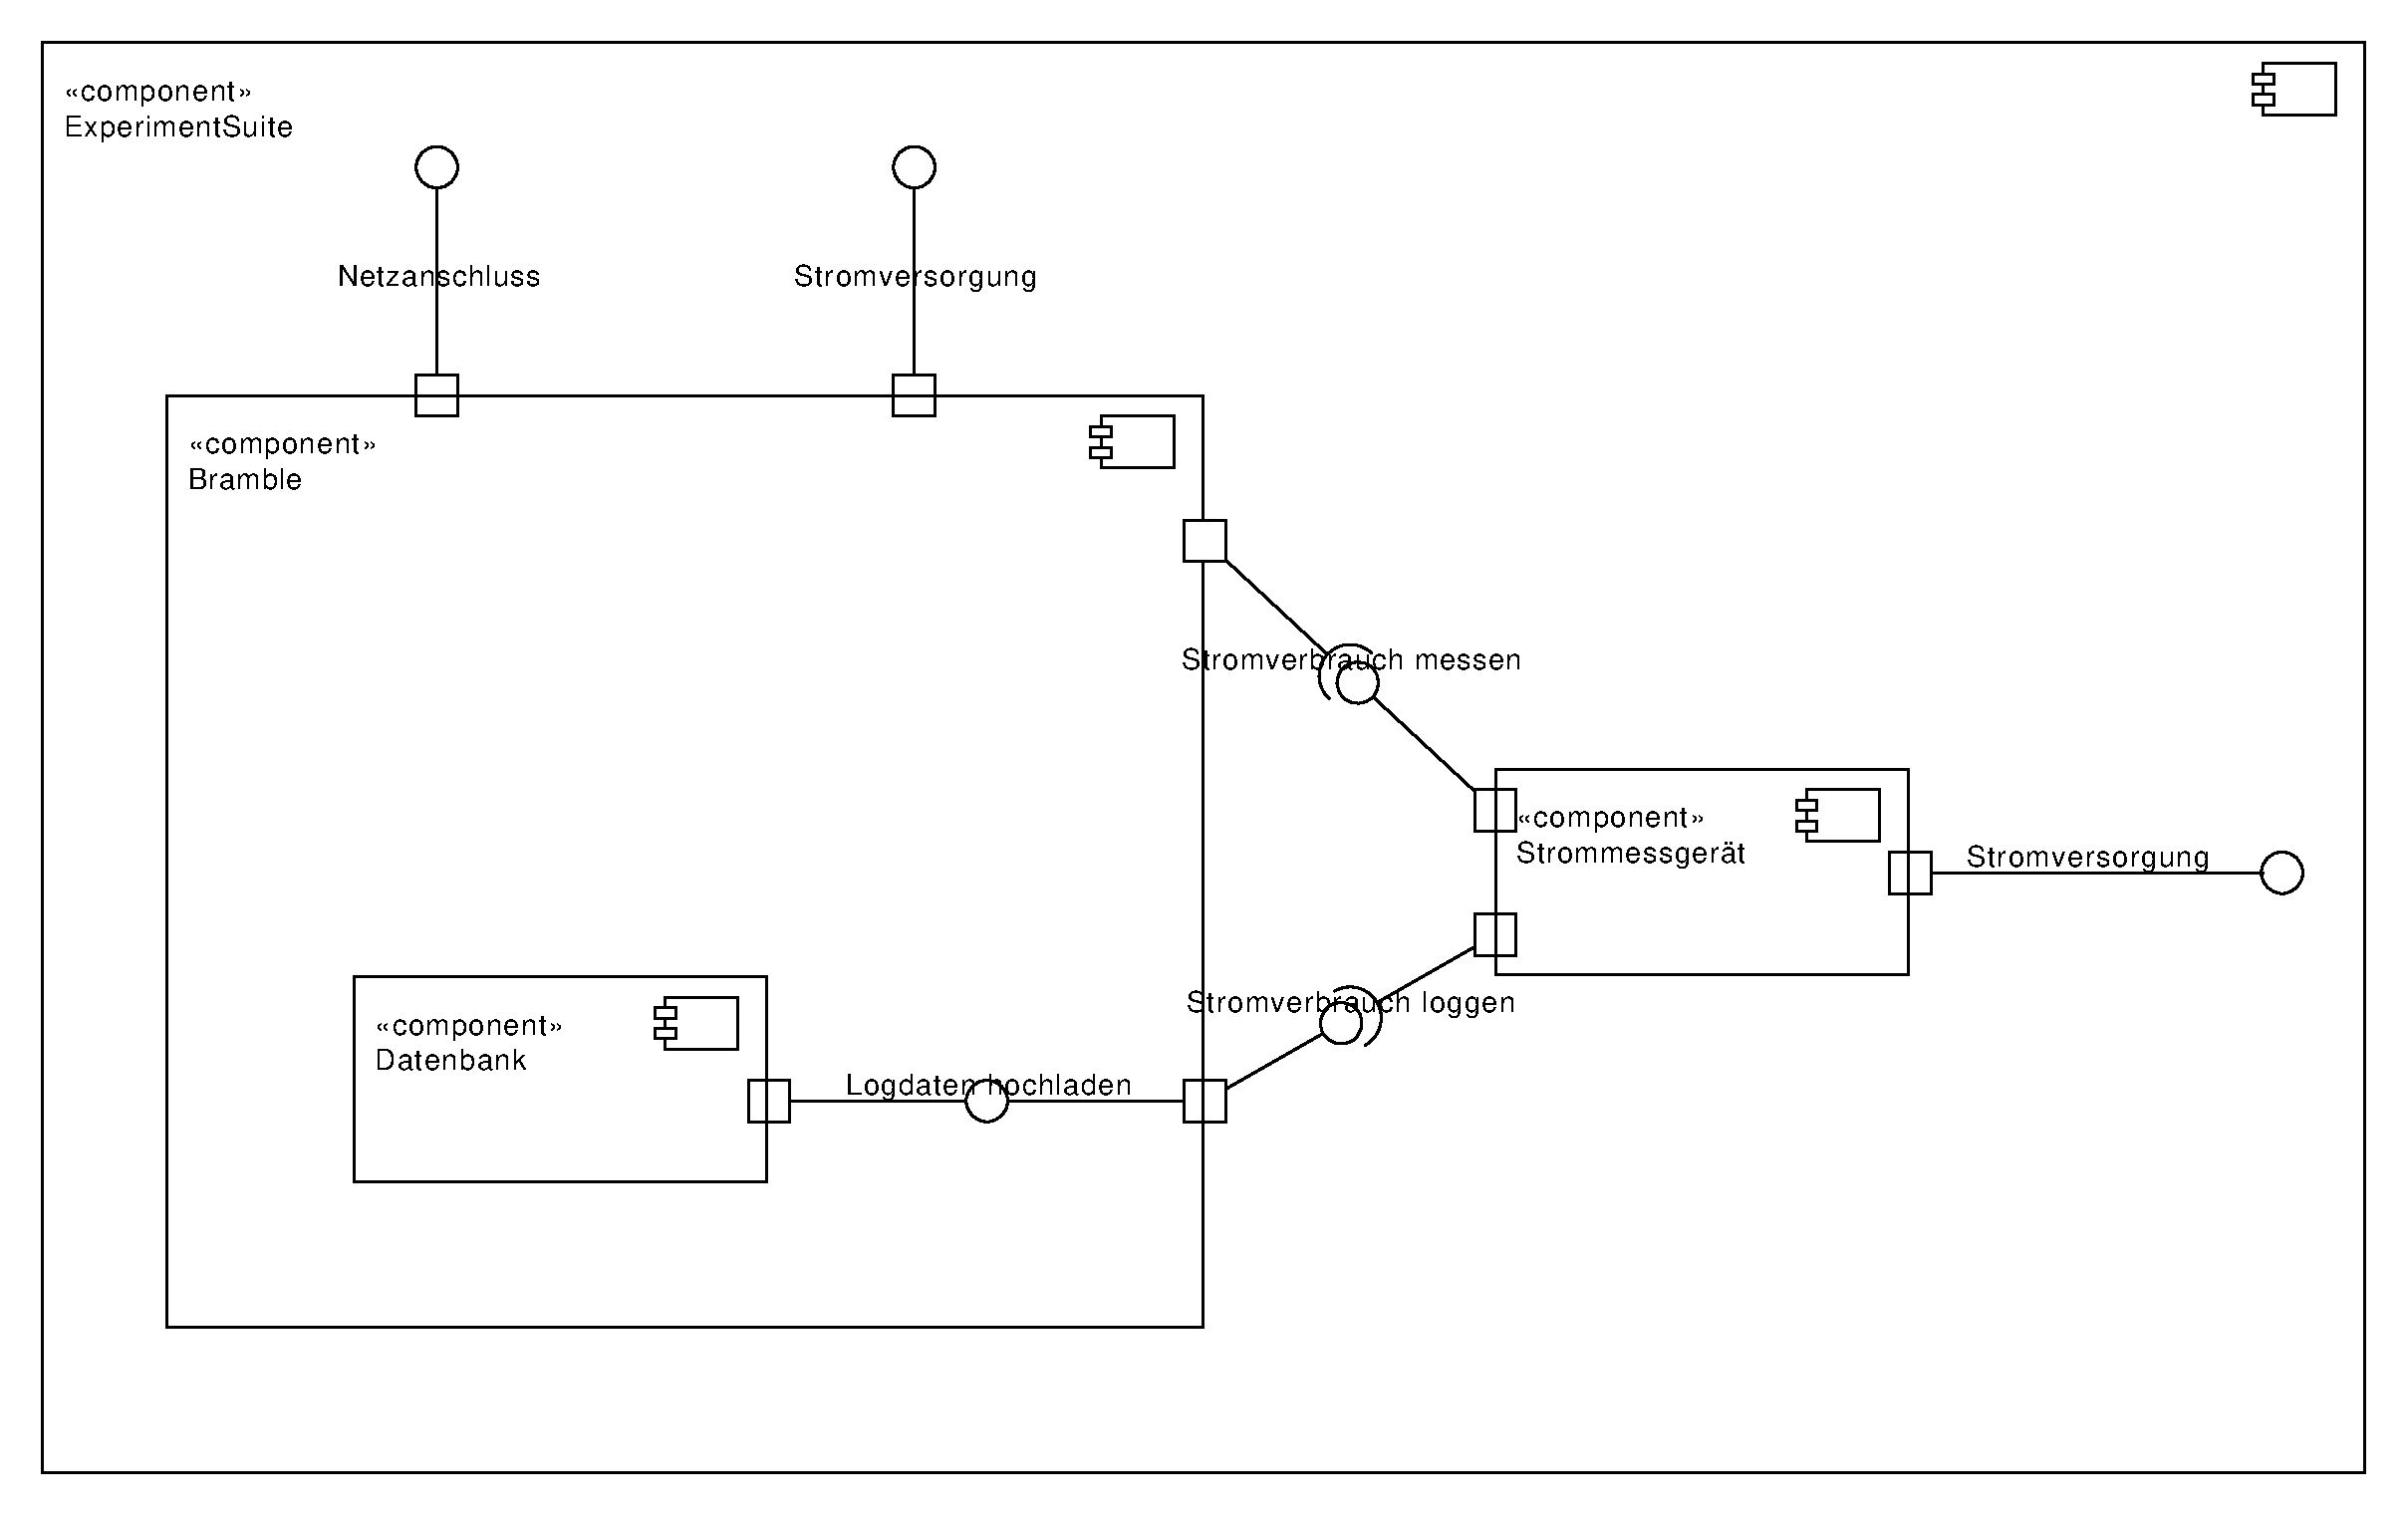
\includegraphics[scale=0.5]{komponentendiagramm2.pdf}} 
  \caption{Komponentendiagramm des Versuchsaufbaus.}
  \label{fig:Komponentendiagramm}		
\end{figure}
\subsubsection{Modifikation der RPi-Knoten}

Zu Beginn der Untersuchung zeigte sich, dass einige Mini-USB-Kabel zur Stromversorgung der RPis defekt waren. Sie wurden durch funktionsf"ahige Kabel ersetzt. 

\subsubsection{Zeitsynchronisation der RPi-Knoten} 

Der RPi-Einzelrechner besitzt aus Kostengr"unden keine Systemuhr (vgl. \cite{schmi13}), sondern synchronisiert sich beim Booten gegen einen NTP-Server im Internet. F"ur die parallele Ausf"uhrung eines Programms auf mehreren Rechnerkernen ist die Zeitsynchronisation der RPi-Knoten untereinander essentiell. Auf dem Bramble wird das durch einen OpenNTP-Server auf \texttt{careme} realisiert, gegen den sich die RPi-Knoten synchronisieren (vgl. \cite{kli13}). 

\subsubsection{Skalierung der Messung auf $n-4$ RPi-Knoten} 

Die Ausf"uhrung eines Benchmark-Programms mit einer bestimmten Anzahl aktiver und angeschalteter RPi-Knoten wird als \textit{ExperimentSuite} bezeichnet werden. Abbildung \ref{fig:Aktivitaetsdiagramm} zeigt, welche Schritte aus Benutzersicht zu ihrer Durchf"uhrung erforderlich sind. Messreihe 1 beginnt mit der h"ochsten Anzahl aktiver RPi-Knoten begonnen und iteriert einmal "uber alle Knoten. In Messreihe 2 werden nach jedem Iterationsschritt nicht mehr aktive RPi-Knoten abgeschaltet. Jede Ausf"uhrung eines Benchmark-Programms l"auft prinzipell gleich ab, w"ahrend zu Beginn und an Ende spezielle Vorkehrungen zu treffen sind.  
\begin{figure}[htb]
  \centerline{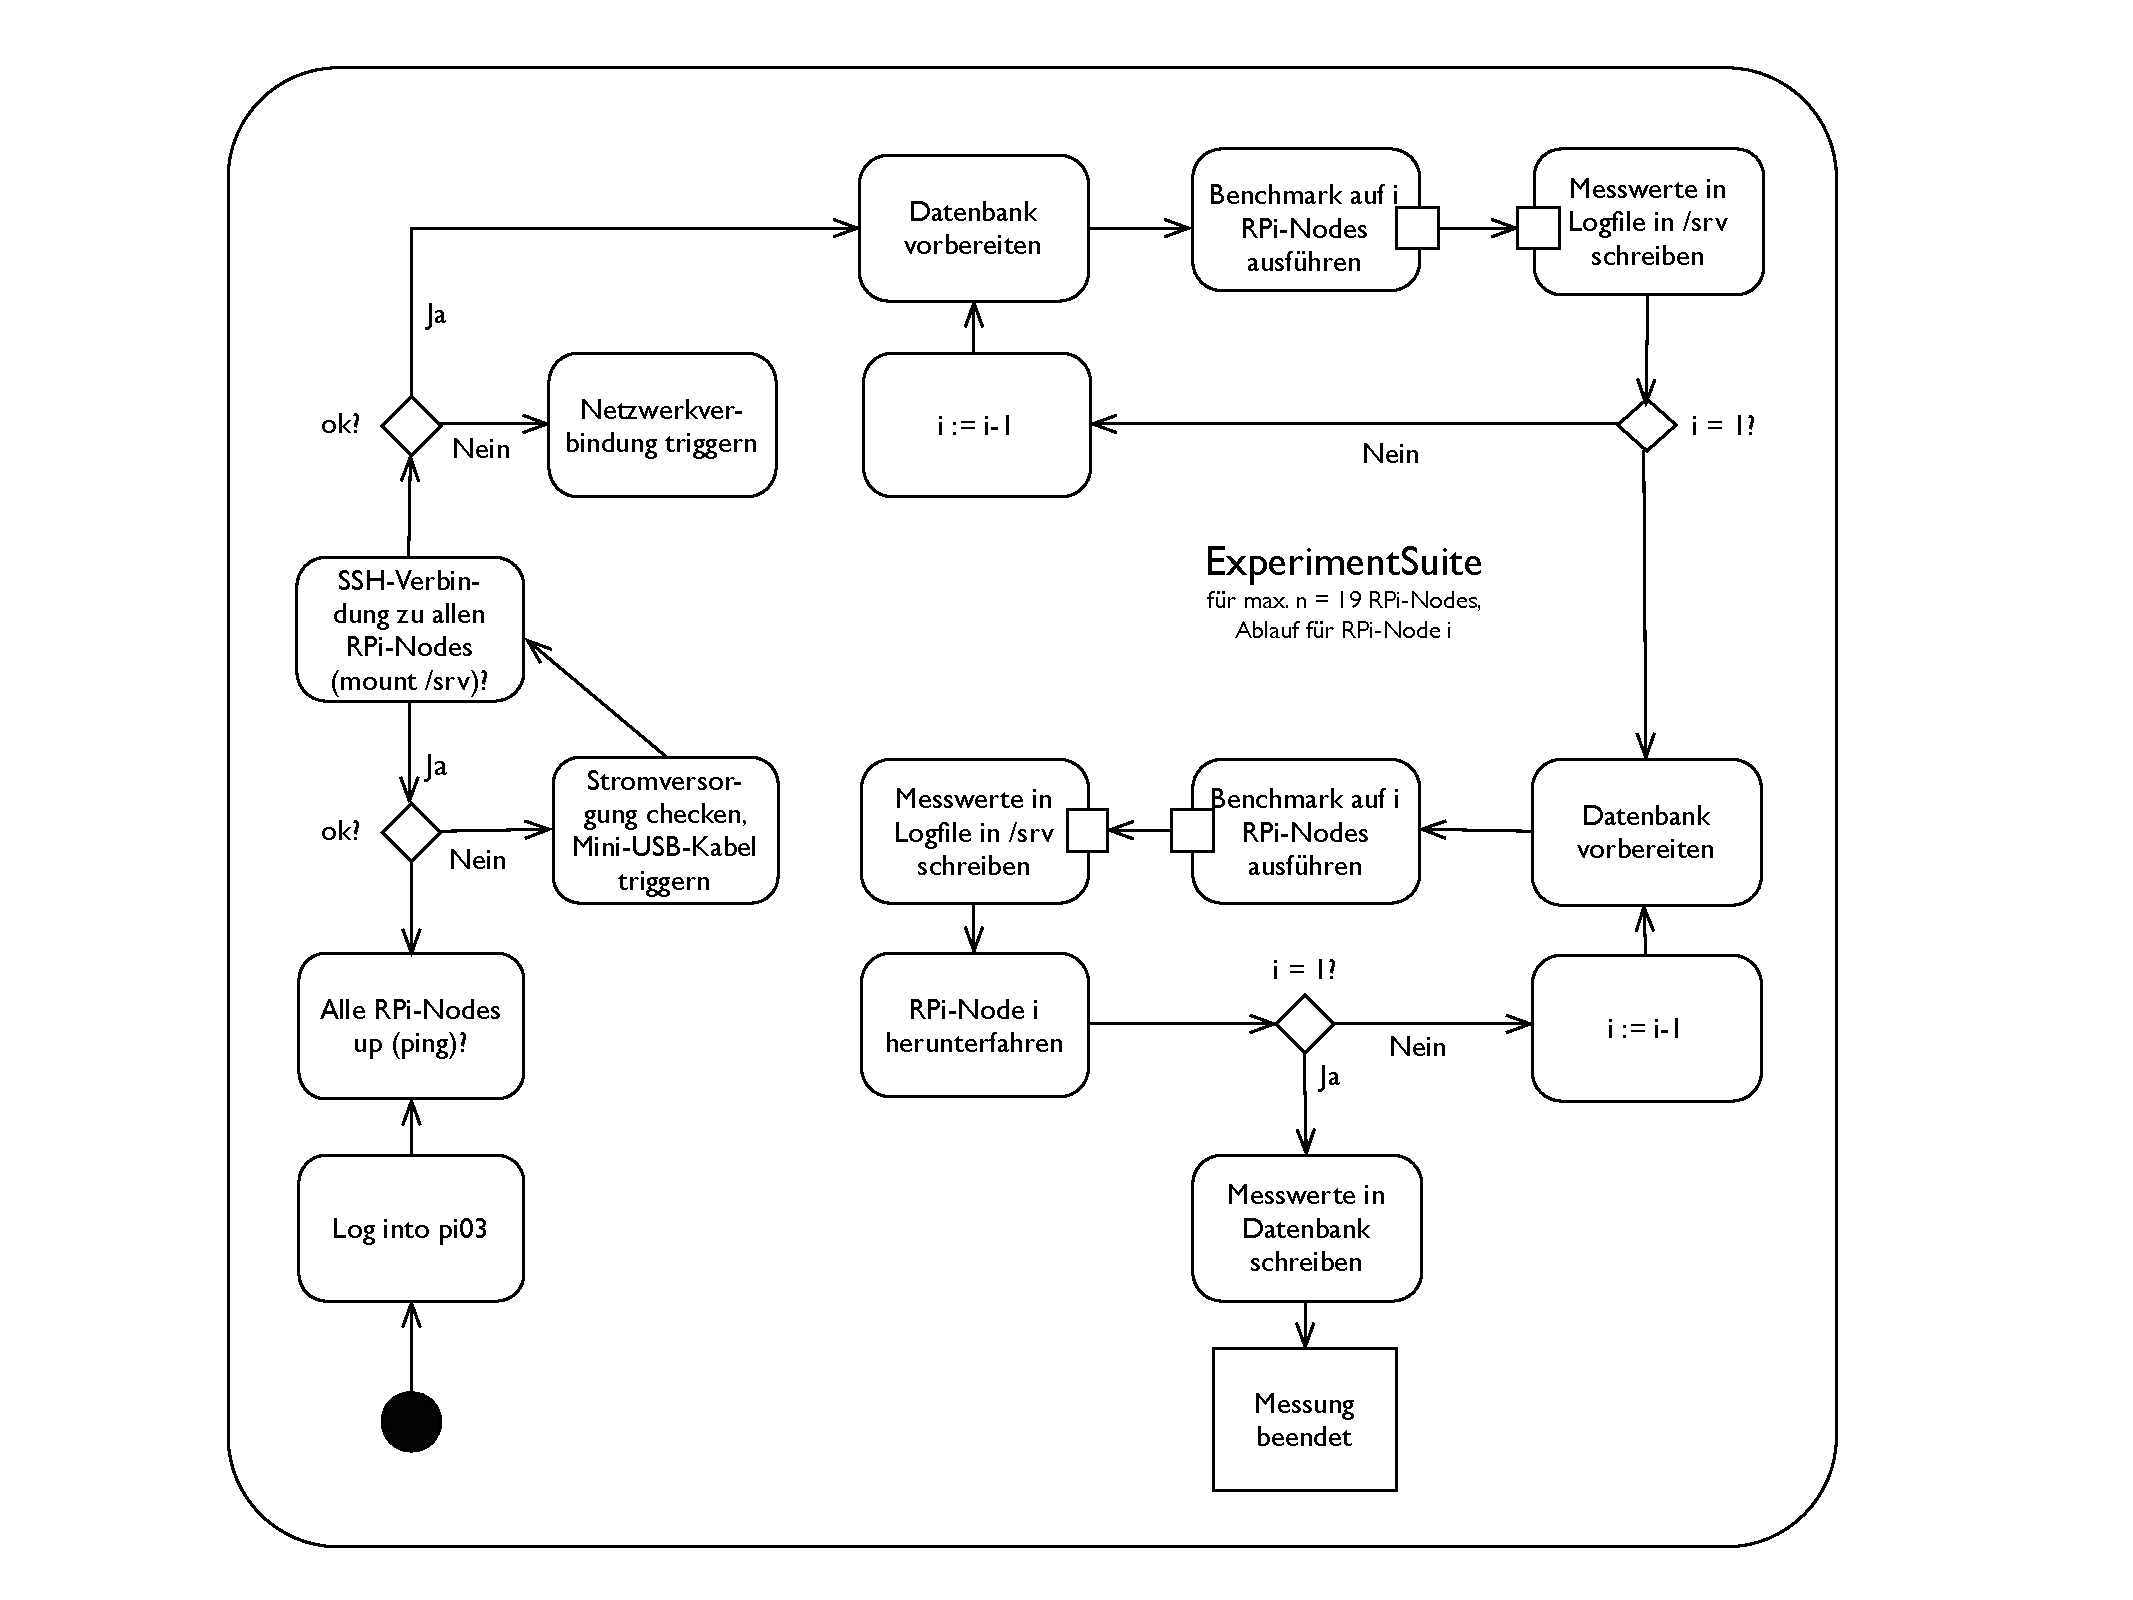
\includegraphics[scale=0.5]{aktivitaetsdiagramm1.pdf}} 
  \caption{Aktivit"atsdiagramm einer ExperimentSuite.}
  \label{fig:Aktivitaetsdiagramm}
\end{figure}

\subsubsection{Konfiguration der Datenbank}

Messergebnisse, Konfigurationen von Benchmarks und ExperimentSuites werden in der My\-SQL-Datenbank \texttt{rpiWerte} auf \texttt{careme} abgelegt. Daf"ur war ein Datenbankschema vorgegeben worden, das die ExperimentSuites in einen gr"o\ss eren Versuchsaufbau integriert. Es wurde w"ahrend der praktischen Arbeit an die tats"achlichen Erfordernisse angepasst: F"ur jedes Modul eines Benchmarks wird ein Messparameter definiert, der Unix-Zeitstempel seines Ausf"uhrungsendes ermittelt und mit dem jeweiligen Messwert in die Datenbank eingelesen. F"ur jede ExperimentSuite werden Anfangs- und Endzeitpunkt als Unix-Zeitstempel ermittelt und in die Datenbank eingelesen. Die Konfiguration erfolgt in vier Schritten:  
\begin{enumerate}%\befseries
	\item Name und Beschreibung des Benchmarks. 
	\item Beschreibung des Versuchsaufbaus. 
	\item Konfiguration des Versuchsaufbaus. 
	\item Verkn"upfung von Benchmark-Konfiguration und Versuchsaufbau.
\end{enumerate} 
Abbildung \ref{fig:Dbconfig1} visualisiert Schritt 1. Die statischen Konfigurationen f"ur STREAM und HPL werden festgelegt. Dazu wurden zwei Shellskripte \texttt{loadGeneratorCon\-figHpl.sh} und \texttt{loadGe\-nerator\-ConfigStream.sh} erstellt. Sie werden zu Beginn des Versuchsaufbaus einmal ausgef"uhrt. Pro Benchmark muss in drei Tabellen jeweils ein Eintrag erstellt werden: In der Tabelle \texttt{LoadGenerator} wird ein Eintrag mit Name und Beschreibung des Benchmarks erstellt. In der Tabelle \texttt{ENUM\_LoadGeneratorConfigura\-tionKey} wird ein Eintrag mit dem Konfigurationsschl"ussel des Benchmarks erstellt. In der Tabelle \texttt{LoadGeneratorConfiguration} wird ebenfalls ein Eintrag mit dem Konfigurationsschl"ussel erstellt.
\begin{figure}[htb]
\centering
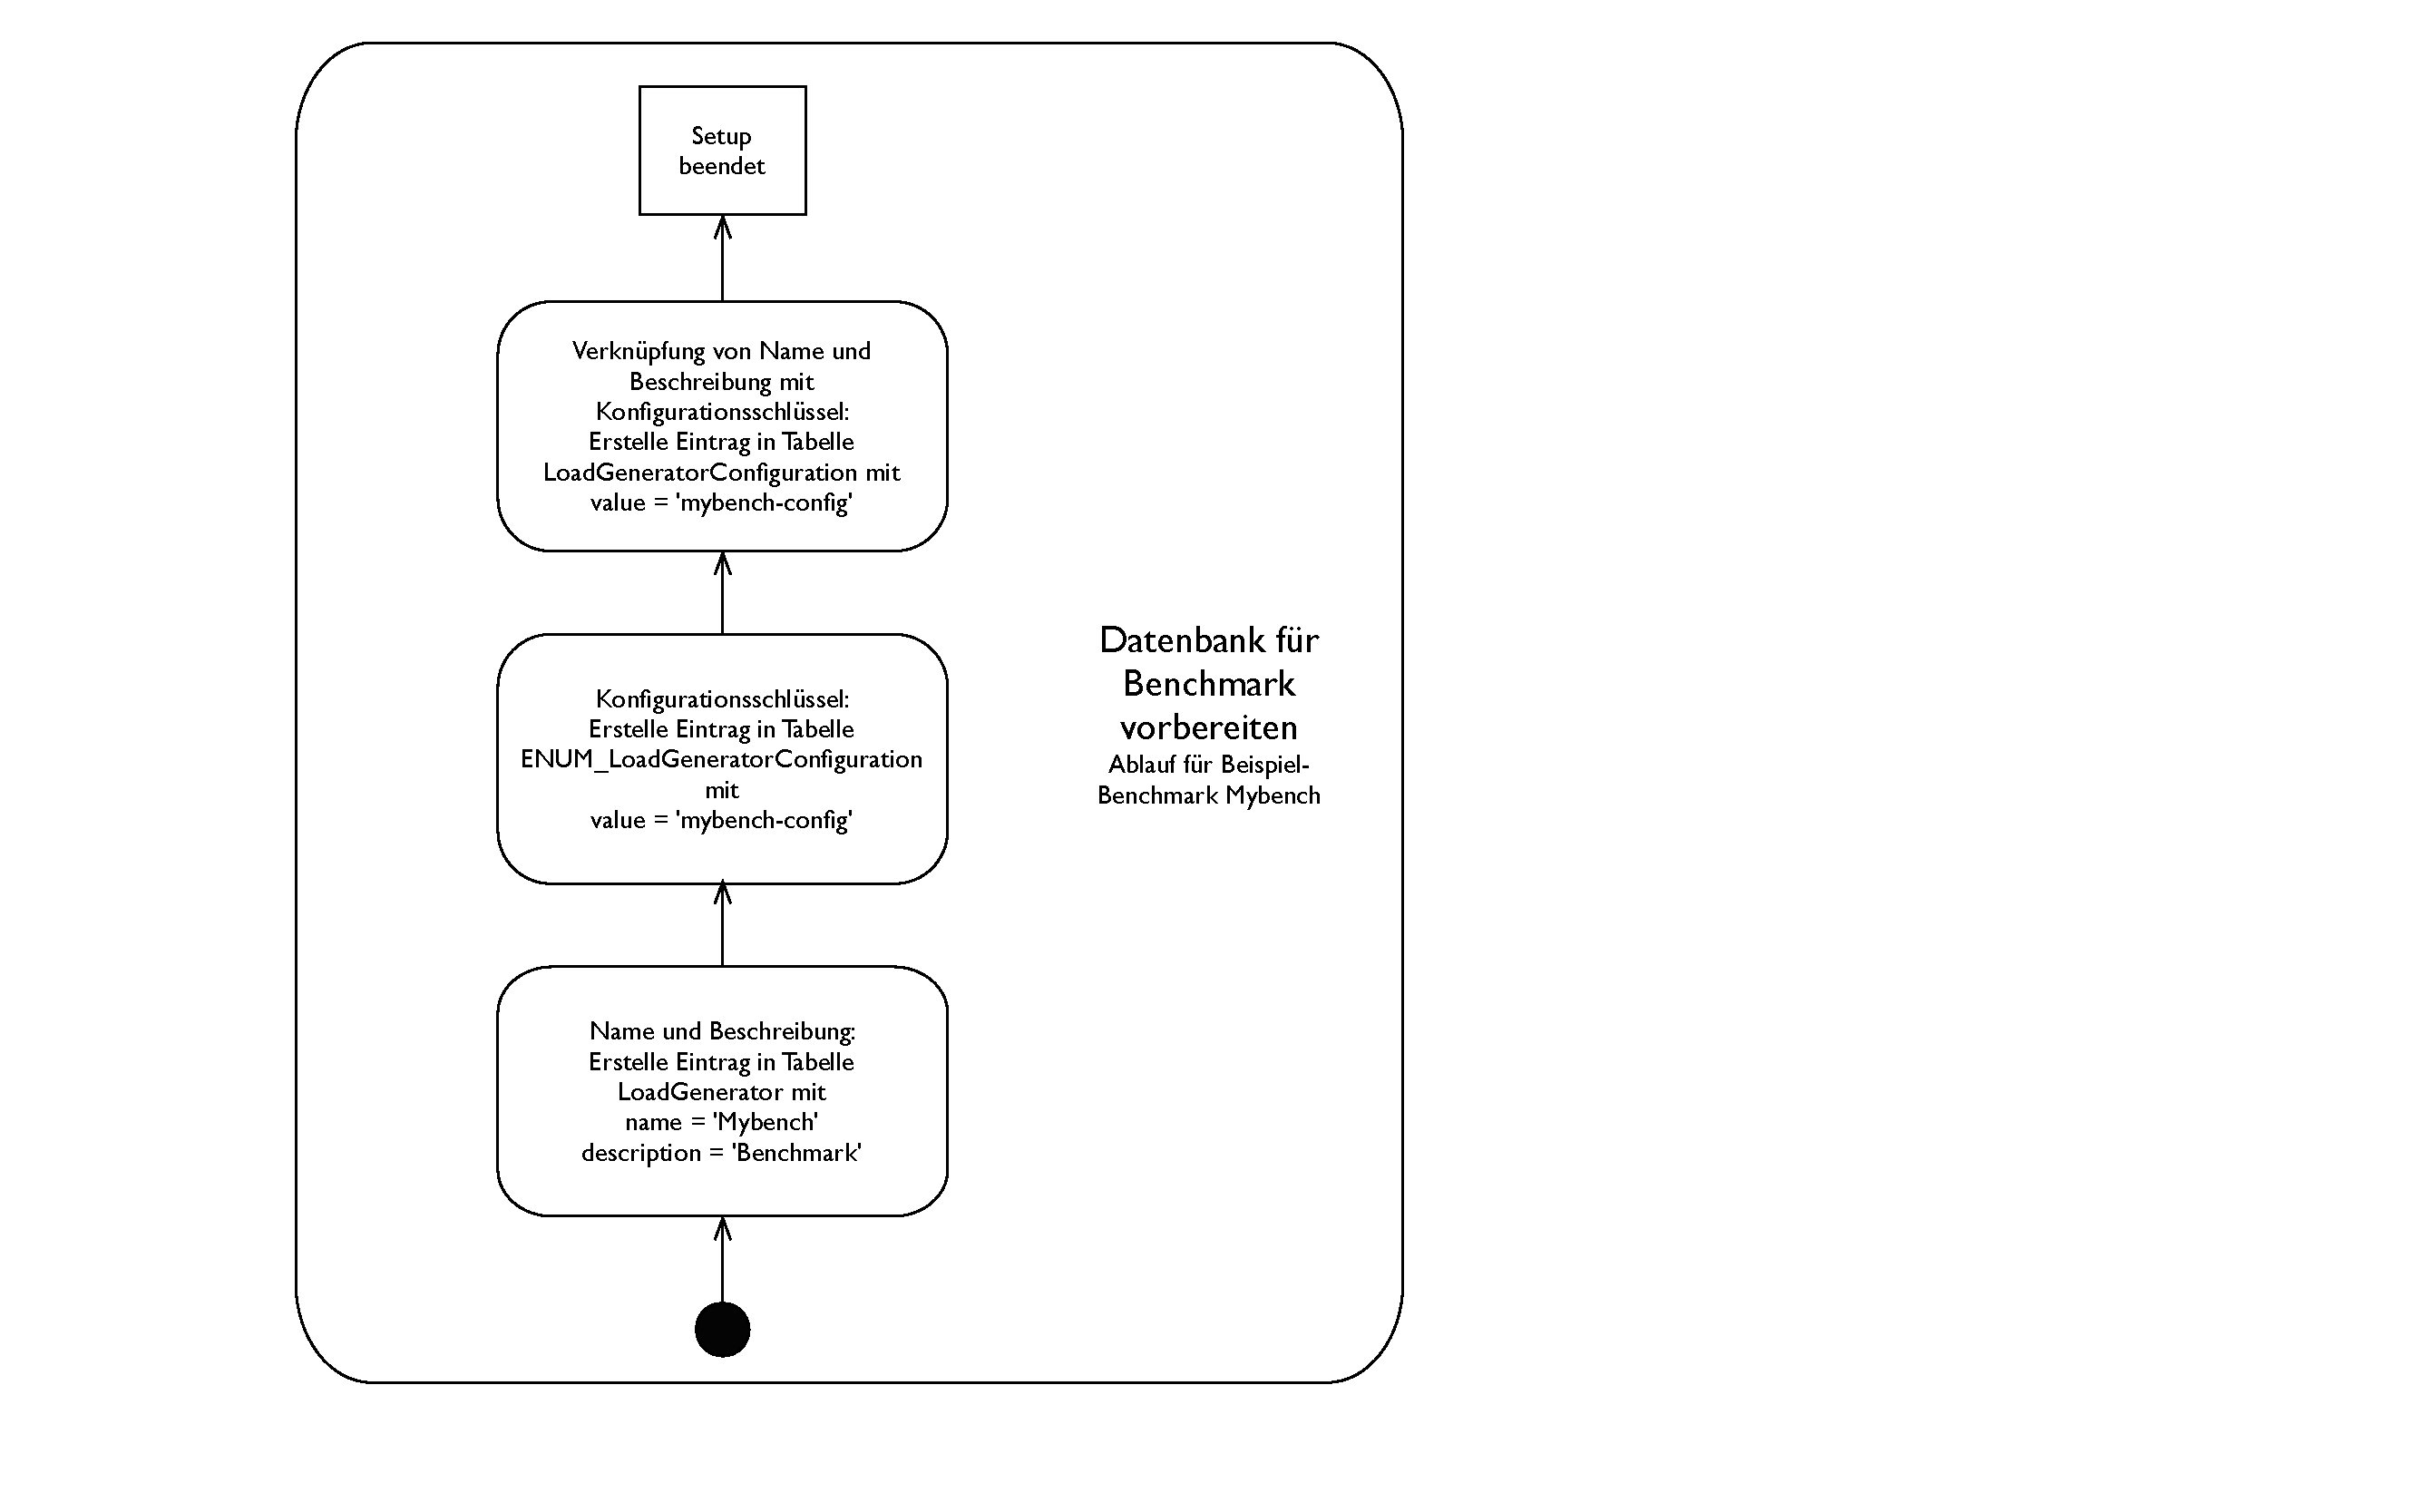
\includegraphics[scale=0.5]{dbconfig1.pdf}
\caption{Aktivit"atsdiagramm zur Konfiguration der Datenbank f"ur einen Benchmark.}
\label{fig:Dbconfig1}
\end{figure}
Die dynamischen Schritte $2-4$ werden einmal pro ExperimentSuite ausgef"uhrt: Name, Beschreibung und Konfiguration des Versuchsaufbaus, Verkn"upfung von ExperimentSuite und Benchmark-Konfiguration. Sie werden in Abbildung \ref{fig:Dbconfig2} veranschaulicht und sind in die Ausf"uhrungsskripte der Benchmarks integriert. 

\subsubsection{Automatisierte Durchf"uhrung der Messung auf $n-4$ RPi-Knoten} 

Die automatisierte Durchf"uhrung der Messung erfolgt durch Shellskripte. Sie werden auf dem Berechnungsknoten \texttt{pi03} ausgef"uhrt und enthalten folgende Schritte: 
\begin{enumerate}\bfseries
	\item Erstellen eines \texttt{Machinefile}, ggf. L"oschen des alten.\\
\normalfont{Zur parallelen Ausf"uhrung eines Programms auf mehreren CPUs durch MPICH wird \texttt{mpiexec} mit dem Parameter \texttt{-machinefile} aufgerufen. Er verweist auf eine Datei, die die Reihenfolge der zu verwendenden CPUs und die Anzahl der darauf auszuf"uhrenden Prozesse spezifiziert. 
\enlargethispage{0.7cm}
Es d"urfen nur so nur so viele Prozesse vergeben werden, wie angeschaltete RPi-Knoten zur Verf"ugung stehen. Die CPUs m"ussen in der Reihenfolge angegeben werden, in der die RPi-Knoten heruntergefahren werden. Ein eventuell veraltetes \texttt{Machinefile} wird gel"oscht.}
	\textbf{\item Einh"angen des geteilten Verzeichnisses auf allen RPis.}\\
Alle Dateien der ExperimentSuites (Binaries, Bibliotheken etc.) liegen im geteilten Verzeichnis \texttt{/srv} bzw. \texttt{/srv/nfs-share}. Daher muss das geteilte Verzeichnis auf jedem verwendeten RPi-Knoten eingeh"angt sein. 
	\textbf{\item Navigation ins Arbeitsverzeichnis.}\\
Alle Shellskripte zur Konfiguration und Ausf"uhrung der ExperimentSuites liegen in einem Verzeichnis \texttt{/srv/experimentsuite}. Die Ergebnisdateien werden ebenfalls dort abgelegt. 
	\textbf{\item Iteration "uber \textit{n} ausgew"ahlte Benchmarks:}
	\begin{enumerate}\bfseries		
		\item Erstellen von Logdateien.\\
\normalfont{F"ur die Ausgabe der Benchmarks werden Logdateien vorbereitet.}  
		\textbf{\item Iteration "uber \textit{n} RPi-Knoten:}
		\begin{enumerate}\bfseries
			\item Datenbank f"ur ExperimentSuite vorbereiten.\\ 
\normalfont{Abbildung \ref{fig:Dbconfig2} visualisiert Schritt b) i. F"ur jede Ausf"uhrung eines Benchmark-Programms wird ein Eintrag in der Tabelle \texttt{ExperimentSuite} mit Granularit"at, Ziel und Startzeitpunkt erstellt. In der Tabelle \texttt{Experiment\-Suite\-Configuration} werden zwei Eintr"age mit Anzahl aktiver und angeschalteter RPi-Knoten erstellt. Beide Tabellen werden "uber die Tabelle \texttt{N2M\_\-loadConf3expSuite} verkn"upft. Darin wird ein Eintrag mit ID des Benchmarks und ID der ExperimentSuite erstellt.}
\begin{figure}[htb]
\centerline{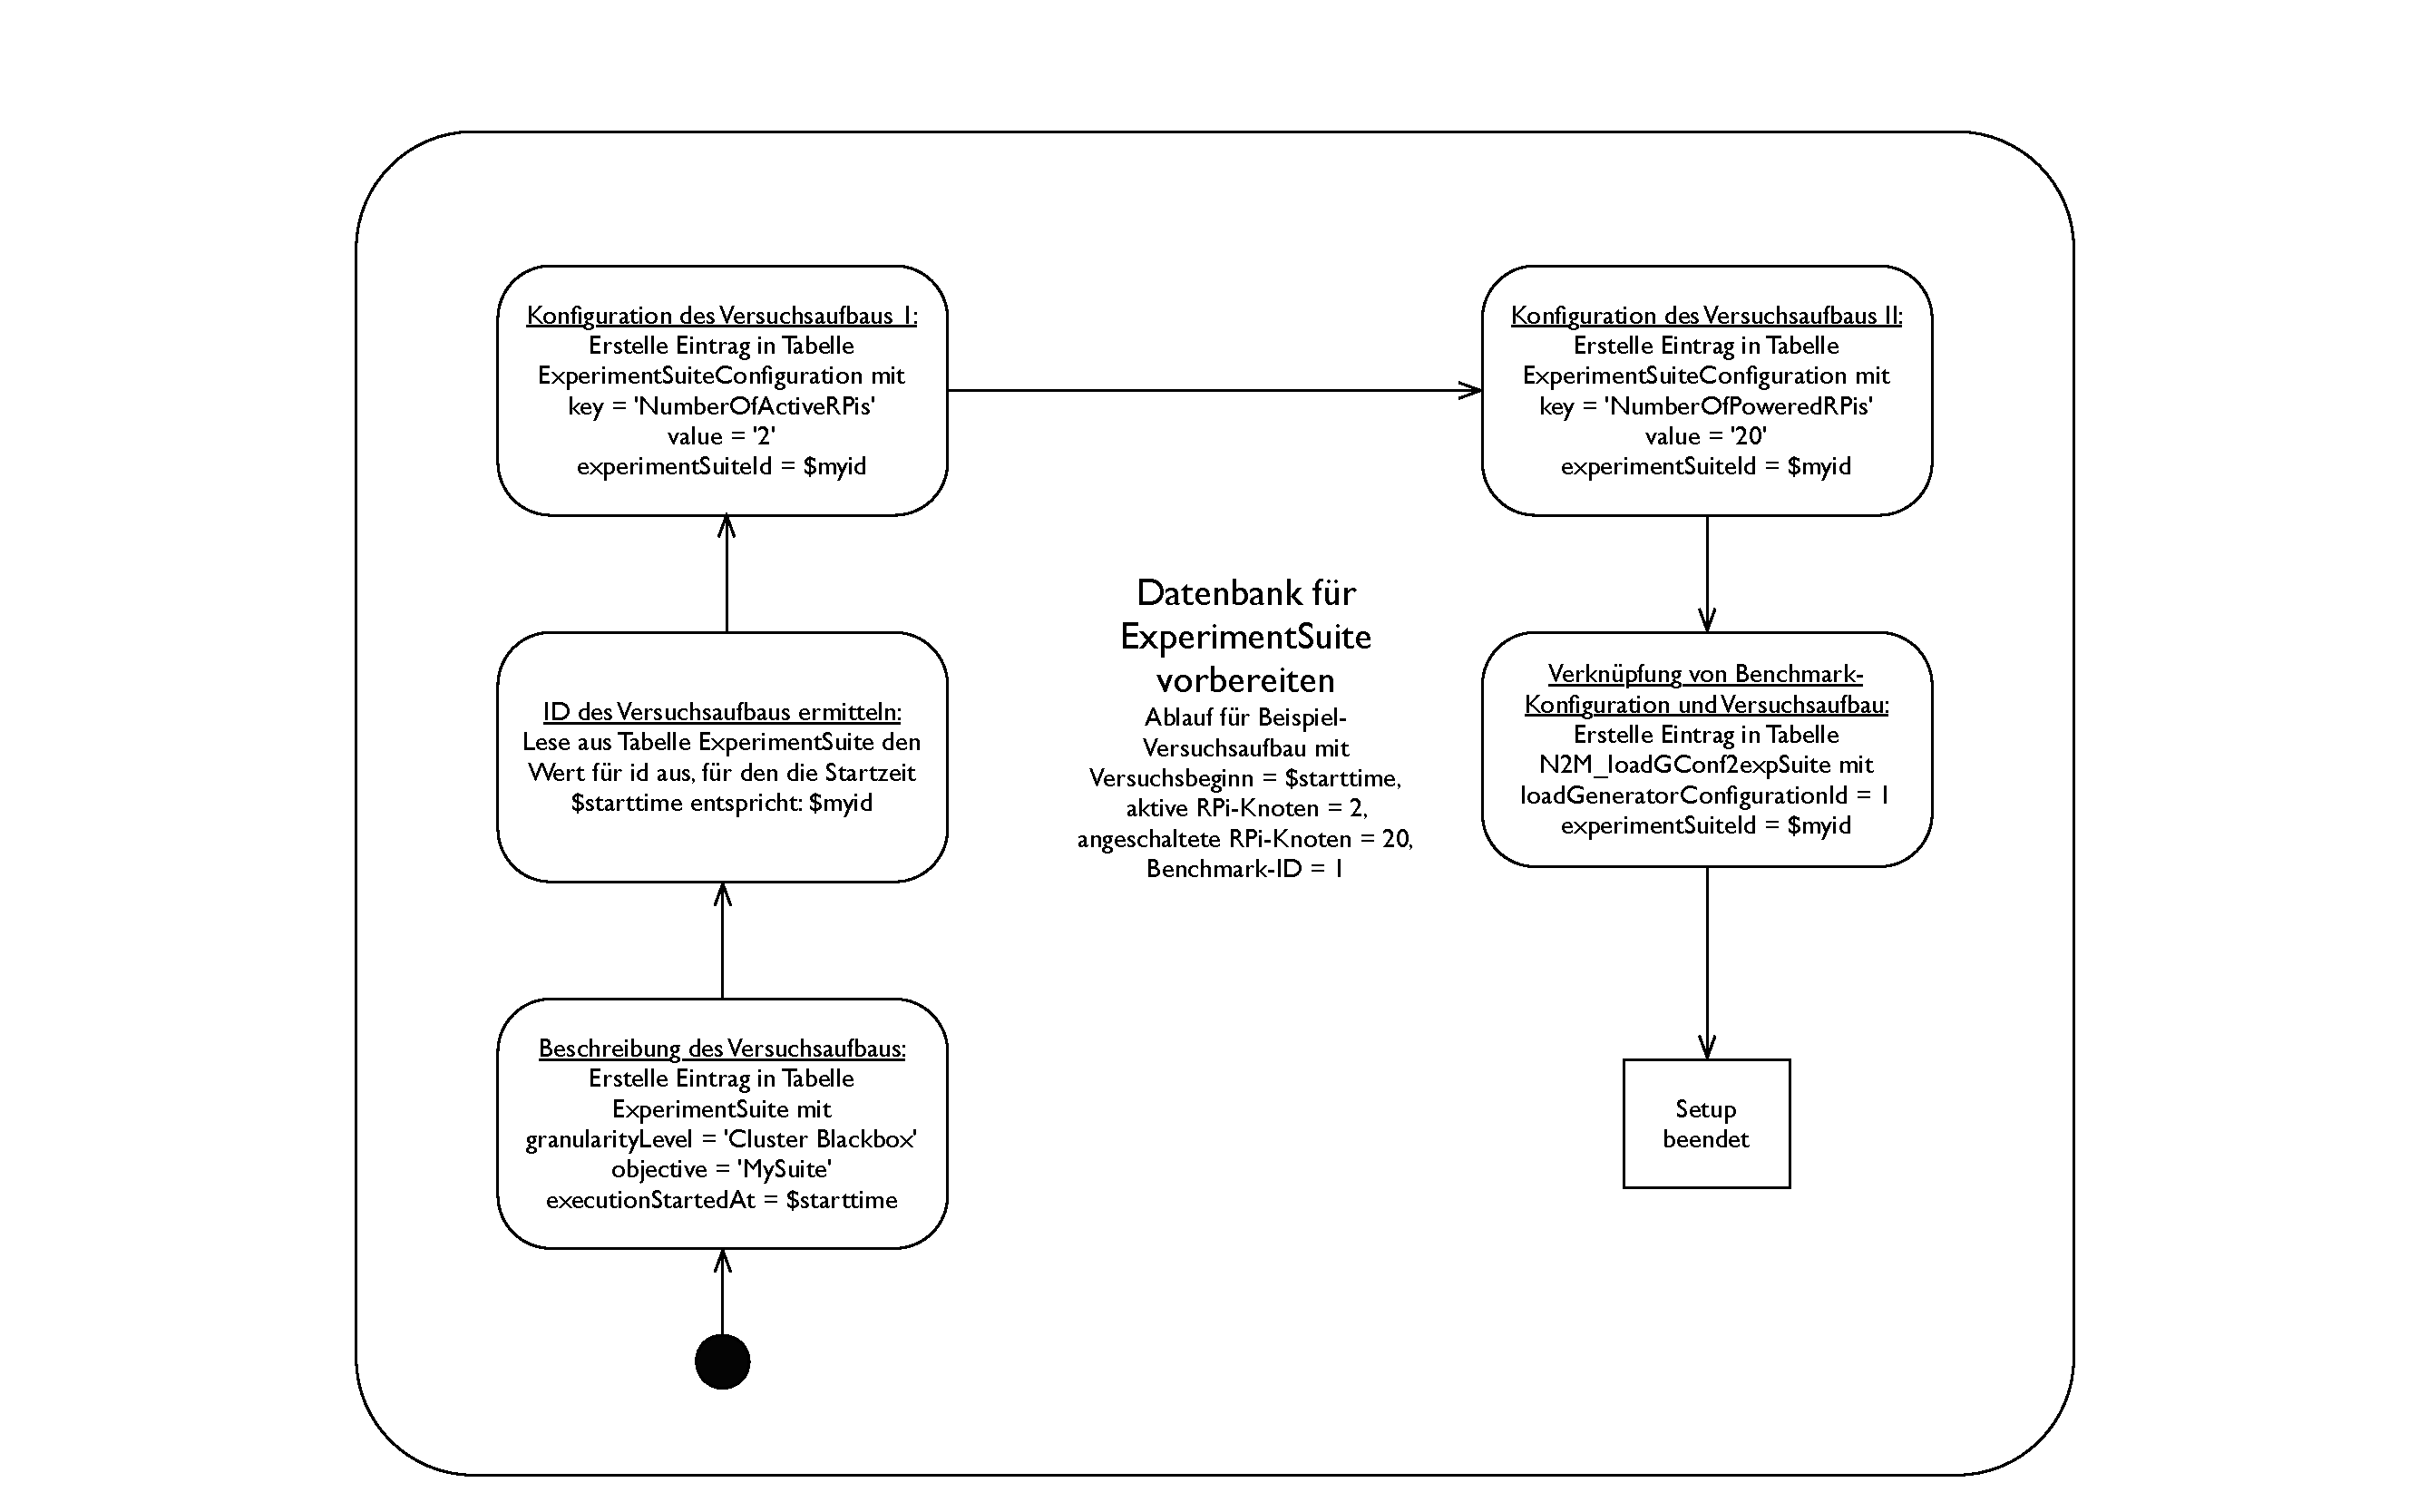
\includegraphics[scale=0.5]{dbconfig2.pdf}}
\caption{Aktivit"atsdiagramm zur Konfiguration der Datenbank f"ur eine ExperimentSuite.}
\label{fig:Dbconfig2}
\end{figure}
			\textbf{\item Parallele Ausf"uhrung auf \textit{n} RPi-Knoten.}\\ 
Zur parallelen Ausf"uhrung ben"otigt \texttt{mpiexec} weitere Parameter: \texttt{-n} spezifiziert die Anzahl an parallelen Programmaufrufen, \texttt{-wdir} das Arbeitsverzeichnis, in das gewechselt werden soll, und \texttt{file} die ausf"uhrbare Datei (vgl. \url{http://www.mpich.org/static/docs/latest/www1/mpiexec.html}). Die parallele Ausf"uhrung von HPL auf vier RPi-Knoten erfolgt z.B. mit
\begin{verbatim}
mpiexec -n 4 -machinefile 
/srv/libraries/etc/mpich-3.0.4-shared/machinefile_latest 
-wdir /srv/benchmarks/bin/hpl-2.1/messung1 
/srv/benchmarks/bin/hpl-2.1/messung1/xhpl >> 
results/hpl-2.1_`date +%y%m%d`.txt
\end{verbatim}
			\textbf{\item Ermittlung des Ausf"uhrungsendes.}\\
Nach der Ausf"uhrung wird der Endzeitpunkt als Unix-Zeitstempel ermittelt. Der entsprechende Eintrag in der Tabelle \texttt{Experiment\-Suite} wird um diesen Wert erg"anzt.
			\textbf{\item Schreiben der Ergebnisdaten.}\\
Die Ausgabe wird in die vorbereitete Logdatei geschrieben. Falls das Bench\-mark-Programm keinen Zeitstempel vorsieht (z.B. STREAM), wird dieser ermittelt und als zus"atzliche Zeile hinzugef"ugt. Damit kann sp"ater f"ur jeden Messwert ein Zeitstempel in die Datenbank eingelesen werden (vgl. Schritte d und e). Auch zum Abgleich der Messergebnisse von Benchmarks und Strommessger"at ist ein Zeitstempel erforderlich (vgl. Kap. \ref{Strommessung}). 
		\end{enumerate}
\newpage
		\textbf{\item Iteration "uber \textit{n} RPi-Knoten:} 
		\begin{enumerate}\bfseries
			\item Datenbank f"ur ExperimentSuite vorbereiten.\\
\normalfont{Die Datenbank wird wie in Schritt b) i. beschrieben vorbereitet. Der Unterschied zu Messreihe 1 besteht in der Anzahl angeschalteter RPi-Knoten ($n+1$ statt 20).} 
			\textbf{\item Parallele Ausf"uhrung des auf n RPi-Knoten.}\\
Analog zu Schritt b) ii..
			\textbf{\item Ermittlung des Ausf"uhrungsendes.}\\
Analog zu Schritt b) iii..
\newpage
			\textbf{\item Herunterfahren nicht mehr aktiver RPi-Knoten.}\\
In Messreihe 2 werden nicht mehr aktive RPi-Knoten heruntergefahren. Davon ausgenommen ist der Berechnungsknoten \texttt{pi03}. 
			\textbf{\item Schreiben der Ergebnisdaten.}\\ 
Analog zu Schritt b) iv..
		\end{enumerate}
		\textbf{\item Parsen der Logdateien f"ur die Datenbank-Eingabe.}\\
Die Ausgabe der Benchmark-Programme entspricht nicht dem Eingabeformat f"ur die Datenbank. Daher wird pro Benchmark eine Datenbank-Eingabedatei erstellt. Sie enth"alt pro ExperimentSuite eine Zeile mit Messwerten und Zeitstempel.

\noindent
Eine Beispielzeile f"ur STREAM: 
\begin{verbatim}
Copy: 3649.3 0.167595 0.166607 0.168846 Scale: 3428.0 0.178749 
0.177361 0.180439 Add: 4749.8 0.192614 0.192010 0.193745 Triad: 
4630.1 0.197780 0.196974 0.199436 Unixtime: 1396608095
\end{verbatim} 
Eine Beispielzeile f"ur HPL: 
\begin{verbatim}
WR00L2L2 29 1 2 2 0.09 1.965e-04 HPL_pdgesv() end time Wed Mar 
26 15:39:05 2014
\end{verbatim} 
		\textbf{\item Messergebnisse in Datenbank einlesen.}\\
Falls die Zeitstempel in der Datenbank-Eingabedatei noch nicht dem Format des Unix-Zeitstempels entsprechen (vgl. \url{http://unixhelp.ed.ac.uk/CGI/man-cgi?date}), werden sie konvertiert. F"ur jeden Messwert wird ein Eintrag in der Tabelle \texttt{Measure\-mentValue} mit Parameter, Messwert, Zeitstempel und ID der ExperimentSuite erstellt. 		
	\end{enumerate}
\end{enumerate}
\noindent
Zur Durchf"uhrung dieser Schritte wurden die Shellskripte \texttt{startBenchmarks.sh}, \texttt{STREAM.sh}, \texttt{wrapHpl.sh}, \texttt{hplMessreihe1.sh} und \texttt{hplMessreihe2.sh} erstellt.

\section{Strommessung}\label{Strommessung}
% Name, Beschreibung
Der Stromverbrauch wird mit dem Strommessger"at \textit{Energenie EGM-PWM-LAN} (vgl. \url{http://energenie.com/item.aspx?id=6736&lang=de}) ermittelt. Es wird im Folgenden als \textit{Energenie} bezeichnet. Es wird zwischen Steckdose und Bramble angebracht und "uber ein LAN-Kabel mit dem Netzwerk verbunden. 

% Aktivierung
F"ur den Versuchsaufbau war dem Energenie eine statische IP-Adresse zugewiesen und ein DNS-Eintrag erstellt worden. Damit kann im lokalen Netzwerk auf das Ger"at und die ermittelten Messwerte zugegriffen werden. Der Zugriff kann unter anderem durch eine Webbrowser- und eine Windows-Anwendung erfolgen. Damit die Software das Ger"at erkennt, muss es sich im selben Subnetz befinden wie der zugreifende Rechner. 

Die Software musste einmalig f"ur die Benutzung des Energenie eingerichtet werden. Dazu wurden nach der Installation des Programms \textit{PowerManager} IP-Adresse und ein Ger"atename eingetragen. In der Webbrowser-Anwendung wurde das Standardpasswort ge"andert und die NTP-Zeitsynchronisation aktiviert. 

% Messgrößen 
\noindent
Das Energenie misst Spannung in Volt, elektrischen Strom in Amp\`{e}re, Leistung in Watt und Arbeit in Kilowattstunden. Die Messgenauigkeit innerhalb des Messbereichs von 50 W -- 2500 W betr"agt $\pm$ 2$\%$ bzw. $\pm$ 1 W (vgl. \url{http://energenie.com/Repository/6736/EGM-PWM-} \url{LAN_manual---fe4469f6-23eb-40be-8c86-e83faf6a2c5b.pdf}). % TODO Messfehler ermitteln 

% Datenzugriff 
F"ur den Versuchsaufbau erwies sich die Webbrowser-Anwendung als ungeeignet. Zwar werden auf einer grafischen Oberfl"ache die jeweils aktuellen Werte f"ur Spannung, elektrischen Strom, Leistung und Arbeit angezeigt, doch es k"onnen keine Messwerte f"ur eine Zeitspanne abgerufen werden. 

Das Programm PowerManager bietet erweiterte Funktionalit"aten, z.B. Export der Messwerte "uber eine Zeitspanne als \texttt{xls}-Datei. Pro Messung werden drei Werte angegeben: Beginn der Messung, Ende der Messung und Leistung in Watt. Au\ss erdem werden die Messwerte in einer SQLite-Datenbank \texttt{database.sqlite} im Verzeichnis \texttt{C:\textbackslash Program Data\textbackslash PowerManagerData\-base} auf der zugreifenden Windows-Maschine abgelegt. Pro Messung werden zus"atzliche Werte abgelegt wie Widerstand in Ohm und Frequenz in Hertz. F"ur die ExperimentSuites sind die Eintr"age \texttt{Stamp} (Zeitstempel als Integer-Wert) und \texttt{P} (Leistung in Watt als Double-Wert) in der Tabelle \texttt{LogValues} von Bedeutung. Die Entscheidung f"ur das Auslesen der SQLite-Datenbank gegen"uber dem \texttt{xls}-Export fiel wegen der feineren Granularit"at der Zeitstempel. 

% Setup für ExperimentSuite 
Abbildung \ref{fig:energenie} zeigt, welche Schritte aus Benutzersicht pro ExperimentSuite zur Strommessung notwendig sind: 
\begin{figure}[H]
  \centering
  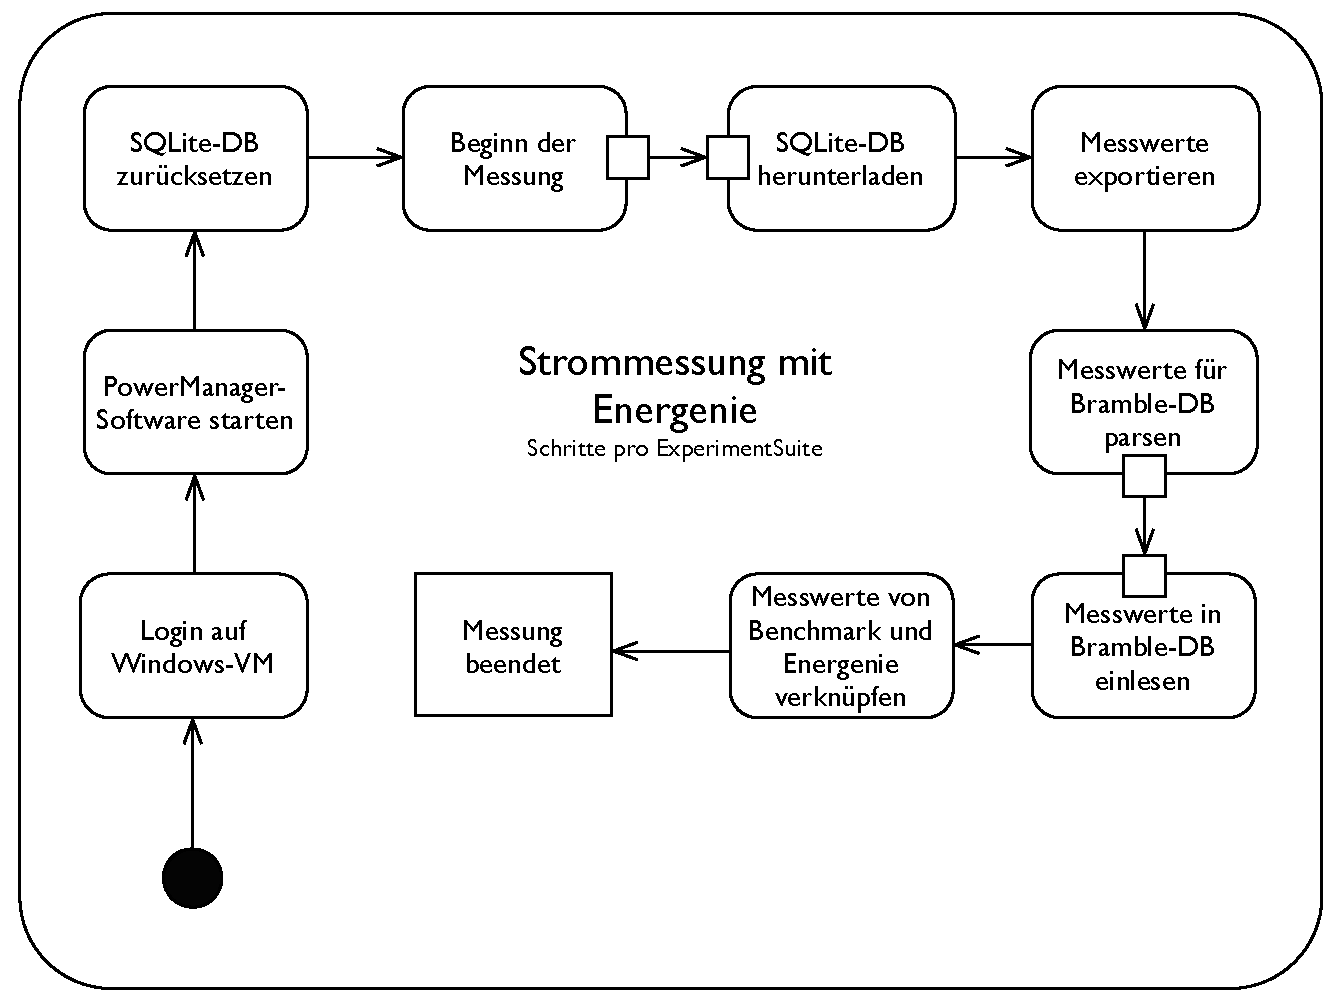
\includegraphics[scale=0.7]{energenie.pdf}\\ 
  \caption{Aktivit"atsdiagramm der Strommessung f"ur eine ExperimentSuite.}
  \label{fig:energenie}		
\end{figure}
\begin{enumerate}\bfseries
% Login auf VM 
	\item Login auf Windows-Maschine.\\
\normalfont
Das Programm PowerManager wird nur f"ur ein Windows-Betriebssystem (Windows XP oder h"oher) angeboten. F"ur die Ausf"uhrung war eine virtuelle Windows-Maschine (Windows 7) im lokalen Netzwerk zur Verf"ugung gestellt worden. 
% PowerManager starten 
	\textbf{\item Start der PowerManager-Software.}
% Grafische Aufzeichnung starten
	\textbf{\item Start der grafischen Aufzeichnung.}\\ 
Optional ist es m"oglich, die aktuellen Messwerte f"ur die Leistung auf einer grafischen Oberfl"ache anzeigen zu lassen. Es hat sich zur "Uberwachung der Messung als sinnvoll erwiesen.
% SQLite-DB herunterladen 
\textbf{\item Herunterladen der SQLite-Datenbank.}\\ 
Zur weiteren Verarbeitung der Messwerte wird die Datenbank von der Windows-Maschine heruntergeladen.
% Export der Messwerte
	\textbf{\item Export der Messwerte.}\\
Zur weiteren Verarbeitung der Messwerte wird die Tabelle \texttt{LogValues} exportiert.	
% Messwerte parsen für MySQL-DB rpiWerte
	\textbf{\item Parsen der Messwerte f"ur MySQL-Datenbank.}\\
Zum Einlesen der Messwerte in \texttt{rpiWerte} m"ussen sie in ein passendes Format gebracht werden. Hierf"ur wurde ein Shellskript \texttt{parseEnergyVa\-lues.sh} erstellt. Es erstellt eine Eingabedatei, die pro Messung eine Zeile mit Leistung und Unix-Zeitstempel enth"alt.
% Messwerte in Bramble-DB einlesen 
	\textbf{\item Einlesen der Messwerte in MySQL-Datenbank.}\\
F"ur jede Messung muss ein Eintrag in der Tabelle \texttt{MeasurementValue} mit Parameter, Messwert, Zeitstempel und ID des Energenie erstellt werden. Hierf"ur wurde ein Shellskript \texttt{writeEnergyValues.sh} erstellt. 
% Messwerte von Strommessung und Benchmarks matchen 
	\textbf{\item Verkn"upfung der Messwerte von Energenie und Benchmark-Programm.}\\ 
Im letzten Schritt m"ussen die Messwerte des Energenie mit den IDs der ExperimentSuites der jeweiligen Messreihe verkn"upft werden. Hierzu wurde ein Shellskript \texttt{matchEnergyValues.sh} erstellt.
\end{enumerate}

\section{Fehlerbehebung}\label{Fehlerbehebung}

W"ahrend der Versuchsdurchf"uhrung zeigten sich Fehlerquellen. Folgende Fehlerf"alle mussten untersucht und behoben werden: 
\begin{enumerate}\bfseries
	\item Defekte Hardware.\\
\normalfont
Neben den defekten Mini-USB-Kabeln hielten mehrere SD-Karten den h"aufigen Schreibzugriffen nicht stand. Sie mussten durch neue SD-Karten ersetzt werden. 
	\textbf{\item RPi-Knoten nicht erreichbar (\texttt{ping}).}\\
H"aufig reagierte ein einzelner RPi-Knoten nicht auf ein \texttt{ping} von einem anderen RPi-Knoten oder von \texttt{careme} aus (Fehlermeldung: \texttt{Destination Host Unreachable}), obwohl die Status-LED Netzwerkaktivit"at anzeigte. Als einzige L"osung erwies sich Ziehen und wieder Einstecken des Mini-USB-Kabels. War das nicht erfolgreich, musste der Vorgang mit dem Netzwerkkabel wiederholt werden. Nach einigen Minuten war der Zielknoten i.d.R. wieder mit \texttt{ping} erreichbar. 
	\textbf{\item RPi-Knoten nicht erreichbar (\texttt{ssh}).}\\ 
Hier traten drei Fehlerf"alle auf: Am h"aufigsten war die Fehlermeldung \texttt{No route to host} beim Versuch, von \texttt{careme} oder einem anderen RPi-Knoten aus eine SSH-Verbin\-dung aufzubauen. Auch hier musste das Netzwerkkabel gezogen und wieder eingesteckt werden. Nach einigen Minuten war der Zielknoten wieder erreichbar. 

Gelegentlich erfolgte ein "uberraschender Passwortprompt f"ur \texttt{root} beim Versuch, eine SSH-Verbindung von einem anderen RPi-Knoten aus aufzubauen. Der RSA Public Key von \texttt{root} musste in die Datei \texttt{\textasciitilde/.ssh/authorized\_keys} auf dem Zielknoten eingetragen werden. 

Gelegentlich erfolgte die Fehlermeldung \texttt{WARNING: REMOTE HOST IDENTIFICATION HAS CHAN\-GED!}. Der RSA Public Key des anfragenden RPi-Knotens musste in der Datei \texttt{\textasciitilde/.ssh/known\_hosts} auf dem Zielknoten korrigiert werden. 
	\textbf{\item Geteiltes Verzeichnis nicht eingeh"angt.}\\ 
Beim Neustart eines RPi-Knotens wurde meist das geteilte Verzeichnis nicht eingeh"angt (Fehlermeldung z.B. \texttt{-bash: /srv/libraries/etc/.sharedprofile: No such file or directory}). Es musste mit \texttt{mount /srv} auf dem betreffenden RPi-Knoten eingeh"angt werden. 
	\textbf{\item Bash-Befehle werden nicht erkannt.} 
Gelegentlich wurden auf einzelnen RPi-Knoten h"aufig verwendete Bash-Befehle nicht erkannt (Fehlermeldung z.B. \texttt{mpiexec: command not found}). Es musste ein Logout und erneuter Login auf dem betreffenden RPi-Knoten erfolgen. 
\end{enumerate}
\noindent 
Der Ausschluss dieser Fehlerf"alle wurde weitestgehend in die Vorbereitung einer ExperimentSuite integriert: "Uberpr"ufung der Netzwerkverbindung aller RPi-Knoten mit \texttt{ping} vom Berechnungsknoten \texttt{pi03} aus, Einh"angen des geteilten Verzeichnisses und damit gleichzeitig die  "Uberpr"ufung der SSH-Verbindung zu allen RPi-Knoten (vgl. Kap. \ref{Bramble-Versuchsaufbau}). 

Spontan auftretende Fehler konnten nicht im Vorfeld ausgeschlossen werden. Die Durchf"uh\-rung einer ExperimentSuite erforderte daher immer die Anwesenheit einer Aufsichtsperson, um z.B. Kabel und Status-LEDs zu "uberpr"ufen. Trat ein spontaner Fehler auf, wurde die Durch\-f"uh\-rung abgebrochen, bereits erstellte Datenbankeintr"age gel"oscht und von Neuem mit den Vorbereitungen begonnen. Auch das Trennen nicht mehr aktiver RPi-Knoten vom Stromnetz musste manuell erfolgen. Jeder Neustart eines RPi-Knoten musste ebenfalls von Hand veranlasst werden, da nur durch Ziehen und erneutes Einstecken des Mini-USB-Kabels ein Neustart erreicht wird (vgl. Kap. \ref{Kap5}). 

Die Messergebnisse wurden dadurch nicht beeinflusst, da eine Messreihe bei St"orungen abgebrochen und von Neuem begonnen wurde. F"ur zuk"unftige Versuchsaufbauten erscheint eine entsprechende Anpassung der Cluster-Architektur sinnvoll (vgl. Kap. \ref{Kap5}).

\section{Ergebnisse}\label{Ergebnisse}

Der folgende Abschnitt stellt die Untersuchungsergebnisse f"ur HPL und STREAM auf dem Bramble dar. Da keine Implementierung von Whetstone f"ur MPICH existiert, war im Verlauf der Untersuchung vorgegeben worden, Whetstone nicht zu ber"ucksichtigen. HPL in der verwendeten Implementierung ben"otigt mindestens vier CPUs oder parallele Prozesse. Hier wurde jeder CPU, d.h. jedem RPi-Knoten, genau ein Prozess zugewiesen. Zur Ausf"uhrung von HPL werden somit mindestens vier angeschaltete und aktive RPi-Knoten ben"otigt. Zur besseren Lesbarkeit wurde die Ausf"uhrung von STREAM daran angepasst. Auch STREAM wurde auf mindestens vier RPi-Knoten parallel ausgef"uhrt. 

\subsection{HPL: Performance}\label{Ergebnisse-HPL}

HPL in der verwendeten Implementierung (vgl. Kap. \ref{Linpack-RPi}) liefert folgende Ausgabe:

Zun"achst werden die verwendeten Eingabe- und Ausgabeparameter erl"autert. Die Ausgabeparameter sind invariabel: \texttt{Gflops} (Ausf"uhrungsrate in GFLOPs) und \texttt{Time} (Ausf"uh\-rungsdauer in Sekunden). \texttt{Gflops} wird auf 3, \texttt{Time} auf 2 Nachkommastellen genau angegeben.

Ein Teil der Eingabeparameter ist invariabel wie \texttt{eps} (Maschinengenauigkeit). Die anderen werden der Datei \texttt{HPL.dat} entnommen, die im selben Verzeichnis wie die ausf"uhrbare Datei liegen muss. Die entscheidenden Eingabeparameter sind Problemgr"o\ss e bzw. Ordnung des zu l"osenden linearen Gleichungssystems \texttt{N}, Blockgr"o\ss e \texttt{NB}\footnote{Die L"osung des linearen Gleichungssystems erfolgt durch L/U-Faktorisierung. Dazu wird eine $n\times n+1$-Koeffizientenmatrix der Ausgangsmatrix \textit{A} erzeugt. \textit{A} wird dazu in in Bl"ocke der Gr"o\ss e \texttt{NB} $\times$ \texttt{NB} aufgeteilt.}, Gr"o\ss e des Prozessnetzes (\texttt{Ps} und \texttt{Qs})\footnote{Die Bl"ocke werden zur Bearbeitung einem Netz aus Prozessoren der Gr"o\ss e \texttt{P} $\times$ \texttt{Q} "ubergeben. \textit{P} bezeichnet die Anzahl von Prozessoren in einer Spalte, \textit{Q} die Anzahl von Prozessoren in einer Zeile des Netzes.}, Panel-Faktorisierungsstrategie \texttt{PFACTs}\footnote{Zur Unterteilung der Matrix in Submatrizen k"onnen drei verschiedene Algorithmen verwendet werden: Links-schauende, rechts-schauende und Crout-Faktorisierung (vgl. \url{http://www.netlib.org/benchmark/hpl/tuning.html}).} und Teilpanel-Faktorisierungsstrategie \texttt{RFACTs}\footnote{Als Teilpanel-Faktorisierungsstrategien werden dieselben Algorithmen angeboten wie f"ur \texttt{PFACTs}.} (vgl. \url{http://www.netlib.org/benchmark/hpl/algorithm.html}). Um m"og\-lichst gute Resultate f"ur die Performance zu erzielen, muss eine sinnvolle Kombination dieser Parameter gefunden werden. Folgende Werte erwiesen sich als sinnvoll: 
\begin{enumerate} 
	\item \texttt{N}: Die Problemgr"o\ss e sollte so gew"ahlt werden, dass der Hauptspeicher zu ca. 80\% mit der Matrix gef"ullt wird. Sie sollte mindestens einige 100 betragen und ein Vielfaches von 96 sein. Bei einer parallelen Ausf"uhrung ist die Gesamtmenge an Hauptspeicher entscheidend. Sie verh"alt sich proportional zu \texttt{N}$^2$. 
	
Wie in Kap. \ref{RPi-Hardware} beschrieben, verf"ugt der RPi "uber 512 MB SDRAM. Wie bei \cite{kli13} dargestellt, werden davon ca. 50 MB durch das Betriebssystem belegt, sodass noch ca. 450 MB pro RPi-Knoten zur Verf"ugung stehen. 

Um die Proportionalit"atskonstante f"ur die Wahl von \texttt{N} zu ermitteln, wurde mit verschiedenen Vielfachen von 96 experimentiert und die Belegung des Hauptspeichers mit \texttt{top} kontrolliert. F"ur $n=4$ RPi-Knoten wurde die beste Performance mit \texttt{N}$=2880$ erzielt. Daraus wurde die Proportionalit"atskonstante als \[k=8294400/1800=4608\] berechnet. Damit ergeben sich folgende Werte f"ur \texttt{N}:

\noindent
$n=4$ RPi-Knoten:\\
Verf"ugbarer Hauptspeicher $=450$ MB$\ast 4=1800$ MB\\
\texttt{N} $=30\ast 96=2880$ (empirisch ermittelt)

$n=8$ RPi-Knoten:\\
Verf"ugbarer Hauptspeicher $=450$ MB$\ast 8=3600$ MB\\
\texttt{N} $=\sqrt{4608\ast 3600}\approx 4073\Rightarrow$ setze \texttt{N} $=42\ast 96=4032$

$n=16$ RPi-Knoten:\\
Verf"ugbarer Hauptspeicher $=450$ MB$\ast 16=7200$ MB\\
\texttt{N} $=\sqrt{4608\ast 7200}=5760\Rightarrow$ setze \texttt{N} $=60\ast 96=5760$	
	\item \texttt{NB}: Die Blockgr"o\ss e wird in Abh"angigkeit von der Cache-Gr"o\ss e gew"ahlt, der m"oglichst vollst"andig gef"ullt werden soll, aber nicht "uberlaufen darf. Es empfiehlt sich eine Quadratzahl zu w"ahlen, ferner ein Vielfaches von 2. 

Der Level 2-Cache von 128 KB des RPi ist f"ur die GPU reserviert (vgl. \url{http://sandsoftwaresound.net/raspberry-pi/memory-hierarchy/}). Um ein "Uberlaufen des Level 1-Datencaches von 16 KB zu vermeiden, wurde \texttt{NB} $= 8$ gesetzt. 
	\item \texttt{Ps} und \texttt{Qs}: Es empfiehlt sich ein m"oglichst quadratisches Prozessnetz zu w"ahlen, ferner ein Vielfaches von 2. Folgende Werte wurden daher gesetzt: 
	
$n=4$ RPi-Knoten: \texttt{Ps} $=2$, \texttt{Qs} $=2$\\ 
$n=8$ RPi-Knoten: \texttt{Ps} $=4$, \texttt{Qs} $=2$\\ 
$n=16$ RPi-Knoten: \texttt{Ps} $=4$, \texttt{Qs} $=4$
	\item \texttt{PFACTs}: Die beste Performance wurde mit \texttt{PFACTs} = Left erzielt. 
	\item \texttt{RFACTs}: Die beste Performance wurde mit \texttt{RFACTs} = Crout erzielt.
\end{enumerate}
Offensichtlich m"ussen f"ur unterschiedliche Anzahlen von Prozessoren unterschiedliche Eingabedateien verwendet werden. Daher wurde f"ur jede HPL-ExperimentSuite ein eigenes Arbeitsverzeichnis erstellt und die ausf"uhrbare Datei zusammen mit der entsprechenden Eingabedatei dort abgelegt. 

Abbildungen \ref{fig:hpl1} und \ref{fig:hpl2} zeigen die Ergebnisse von Messreihe 1. Ausgabeparameter sind Ausf"uhrungsrate in GFLOPs und Ausf"uhrungsdauer in Sekunden, jeweils skaliert auf $16-4$ RPi-Knoten.
\begin{figure}[H]
  \centering
  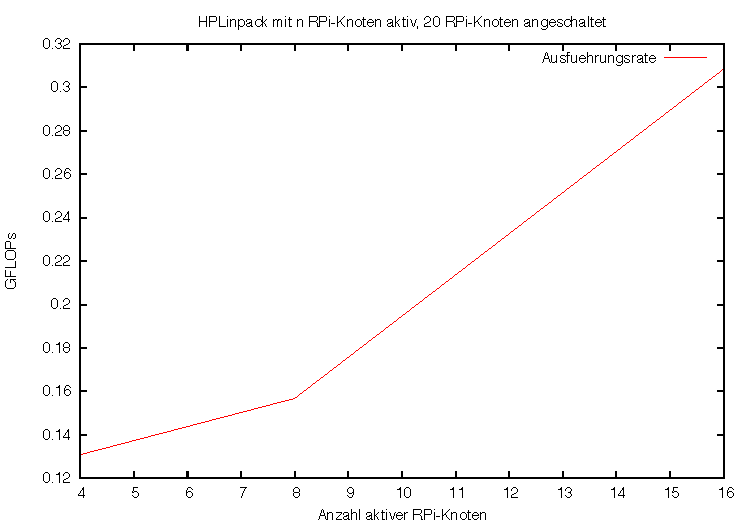
\includegraphics[scale=0.95]{hpl1.pdf}\\ 
  \caption{Ausf"uhrungsrate f"ur HPL, Messreihe 1.}
  \label{fig:hpl1}		
\end{figure}
\begin{figure}[H]
  \centering
  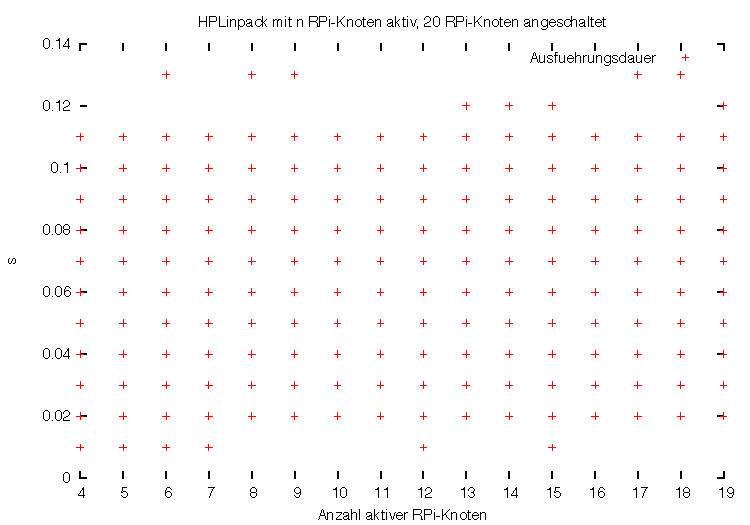
\includegraphics[scale=0.95]{hpl2.pdf}\\ 
  \caption{Ausf"uhrungsdauer f"ur HPL, Messreihe 1.}
  \label{fig:hpl2}		
\end{figure}
%\newpage
\noindent
Abbildungen \ref{fig:hpl5} und \ref{fig:hpl6} stellen die Ergebnisse von Messreihe 1 und Messreihe 2 gegen"uber. Die Ergebnisse von Messreihe 1 sind rot, die von Messreihe 2 blau dargestellt.
\begin{figure}[htb]
  \centering
  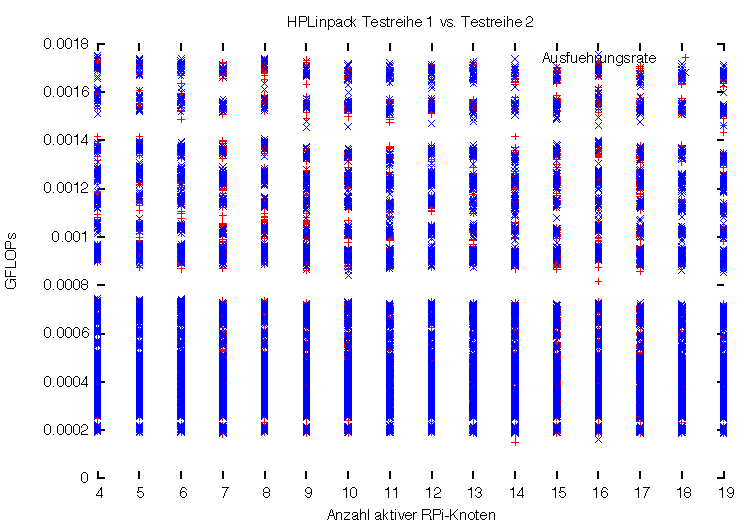
\includegraphics[scale=0.95]{hpl5.pdf}\\ 
  \caption{Ausf"uhrungsrate f"ur HPL, Messreihe 1 und Messreihe 2.}\label{fig:hpl5}
\end{figure}
\begin{figure}[H]
  \centering
  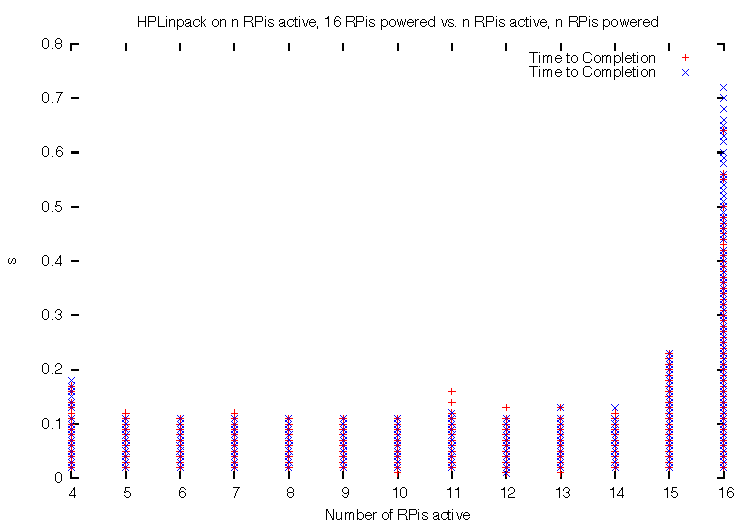
\includegraphics[scale=0.95]{hpl6.pdf}\\ 
  \caption{Ausf"uhrungsdauer f"ur HPL, Messreihe 1 und Messreihe 2.}\label{fig:hpl6}
\end{figure}
%\newpage
\subsection{STREAM: Performance}\label{Ergebnisse-STREAM}
\interfootnotelinepenalty=10000
STREAM in der verwendeten Implementierung (vgl. Kap. \ref{STREAM}) liefert folgende Ausgabe:

Zun"achst erfolgt eine Erl"auterung der verwendeten Eingabe- und Ausgabeparameter. Die wichtigsten Eingabeparameter sind Anzahl an Prozessoren, Vektorl"ange, Speicherbedarf und Anzahl an Iterationen f"ur jedes Modul\footnote{Im Gegensatz zu HPL gibt es keine Eingabedatei, d.h. eine Ver"anderung ist nur direkt im Quellcode m"oglich (vgl. hierzu Kap. \ref{Interpretation-Stream}).}. F"ur die Module Copy, Scale, Add und Triad (vgl. Kap. \ref{Funktion-STREAM}) werden die beste erzielte Ausf"uhrungsrate in MB/s (\texttt{Rate}) und die durchschnittliche (\texttt{Avg time}), minimale (\texttt{Min time}) und maximale Ausf"uhrungsdauer (\texttt{Max time}) in Sekunden ausgegeben. Die Ausf"uhrungsrate wird auf eine, die Ausf"uhrungsdauer auf 6 Nachkommastellen genau angegeben. 

Abbildungen \ref{fig:stream1} und \ref{fig:stream2} zeigen die Ergebnisse von Messreihe 1 f"ur STREAM. Ausgabeparameter sind Ausf"uhrungsrate in MB/s und durchschnittliche Ausf"uhrungsdauer in Sekunden f"ur alle Module, jeweils skaliert auf $19-4$ RPi-Knoten. 
\begin{figure}[htb]
  \centering
  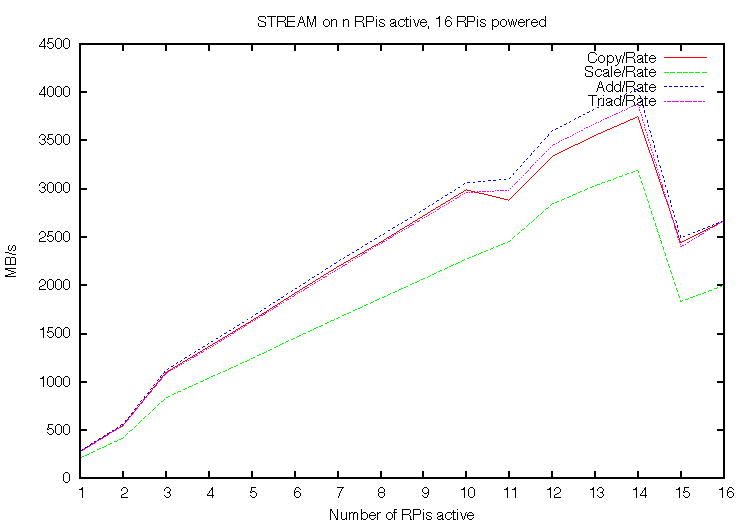
\includegraphics[scale=0.95]{stream1.pdf}\\ 
  \caption{Ausf"uhrungsrate f"ur STREAM, Messreihe 1.}
  \label{fig:stream1}		
\end{figure}
\begin{figure}[H]
  \centering
  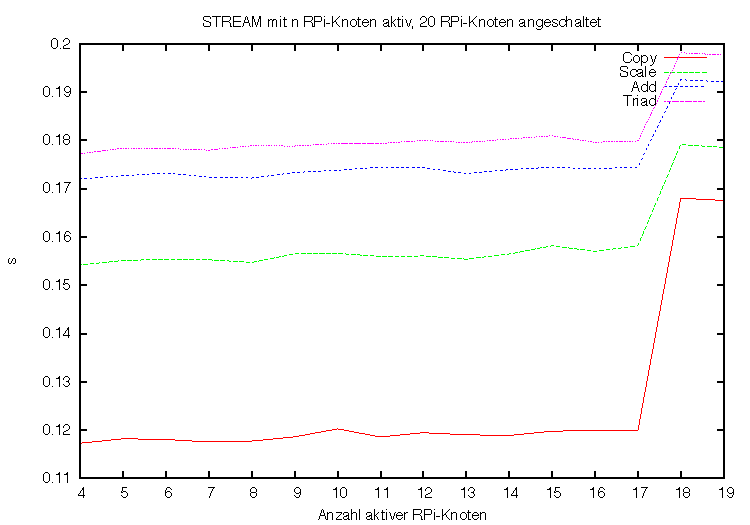
\includegraphics[scale=0.95]{stream2.pdf}\\ 
  \caption{Ausf"uhrungsdauer f"ur STREAM, Messreihe 1.}
  \label{fig:stream2}		
\end{figure}
\newpage
\noindent
Abbildungen \ref{fig:stream5} und\ref{fig:stream6} stellen die Ergebnisse von Messreihe 1 und Messreihe 2 gegen"uber. Die Ergebnisse von Messreihe 1 sind rot, die von Messreihe 2 blau markiert. 
\begin{figure}[htb]
  \centering
  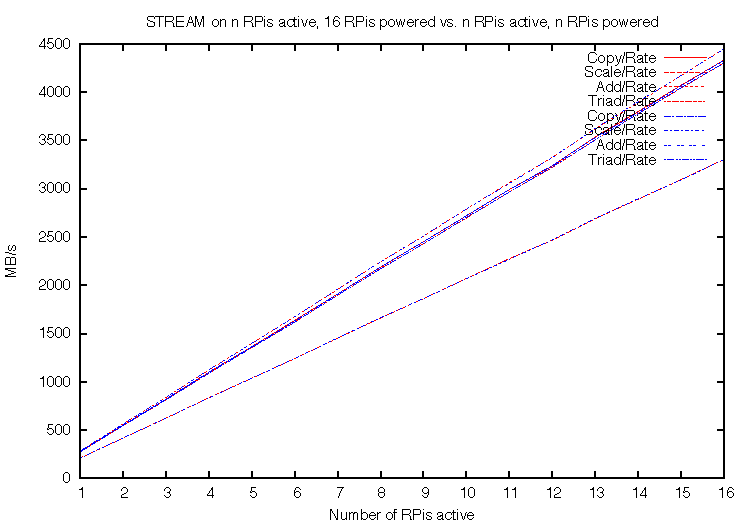
\includegraphics[scale=0.95]{stream5.pdf}\\ 
  \caption{Ausf"uhrungsrate f"ur STREAM, Messreihe 1 und Messreihe 2.}\label{fig:stream5}
\end{figure}
\begin{figure}[H]
  \centering
  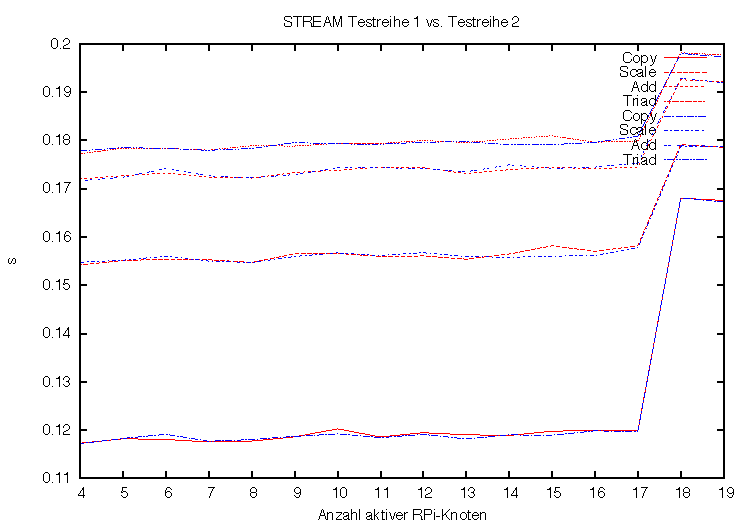
\includegraphics[scale=0.95]{stream6.pdf}\\ 
  \caption{Ausf"uhrungsdauer f"ur STREAM, Messreihe 1 und Messreihe 2.}\label{fig:stream6}
\end{figure}
\newpage
\subsection{Stromverbrauch}\label{Ergebnisse-Energenie}

Abbildungen \ref{fig:strom1} und \ref{fig:strom6} zeigen die Ergebnisse der Strommessung f"ur HPL. Abbildung \ref{fig:strom1} zeigt den Stromverbrauch in Messreihe 1. Abbildung \ref{fig:strom6} stellt den Stromverbrauch von Messreihe 1 und Messreihe 2 gegen"uber. 
\begin{figure}[htb]
  \centering
  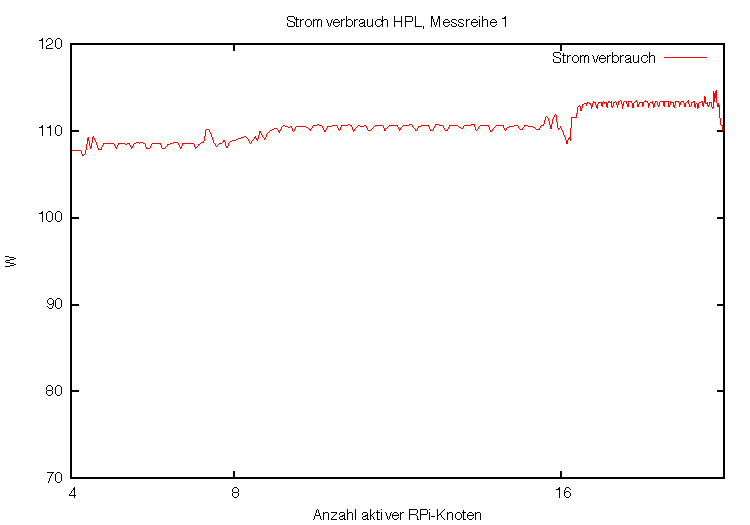
\includegraphics[scale=0.95]{strom1.pdf}\\ 
  \caption{Stromverbrauch f"ur HPL, Messreihe 1.}\label{fig:strom1}
\end{figure}
\begin{figure}[H]
  \centering
  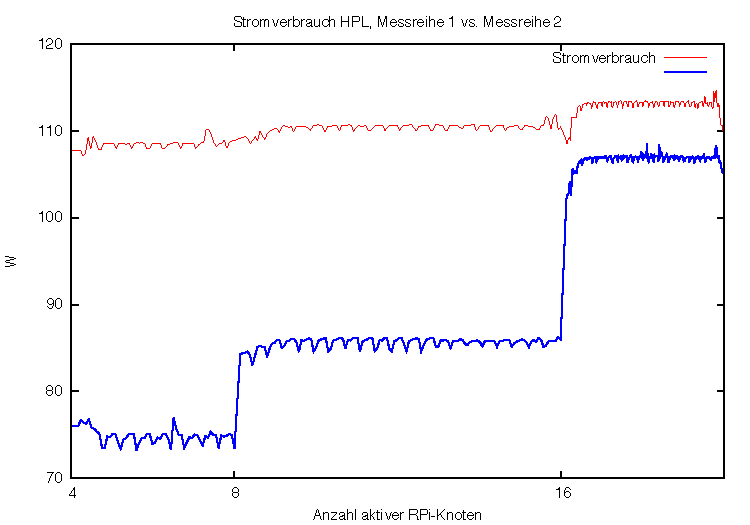
\includegraphics[scale=0.95]{strom6.pdf}\\ 
  \caption{Stromverbrauch f"ur HPL, Messreihe 1 und Messreihe 2.}\label{fig:strom6}
\end{figure}
\newpage
\noindent
Abbildungen \ref{fig:strom3} und \ref{fig:strom5} zeigen die Ergebnisse der Strommessung f"ur STREAM. Abbildung \ref{fig:strom3} zeigt den Stromverbrauch in Messreihe 1. Abbildung \ref{fig:strom5} stellt den Stromverbrauch von Messreihe 1 und Messreihe 2 gegen"uber.
\begin{figure}[htb]
  \centering
  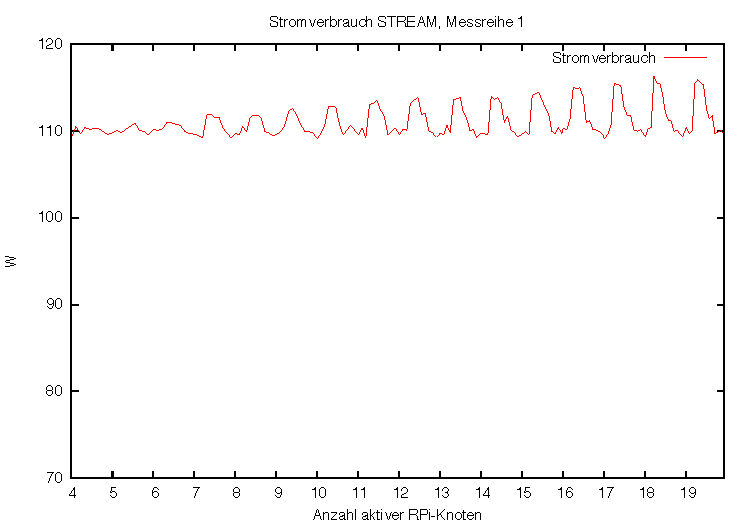
\includegraphics[scale=0.95]{strom3.pdf}\\ 
  \caption{Stromverbrauch f"ur STREAM, Messreihe 1.}\label{fig:strom3}
\end{figure}
\begin{figure}[H]
  \centering
  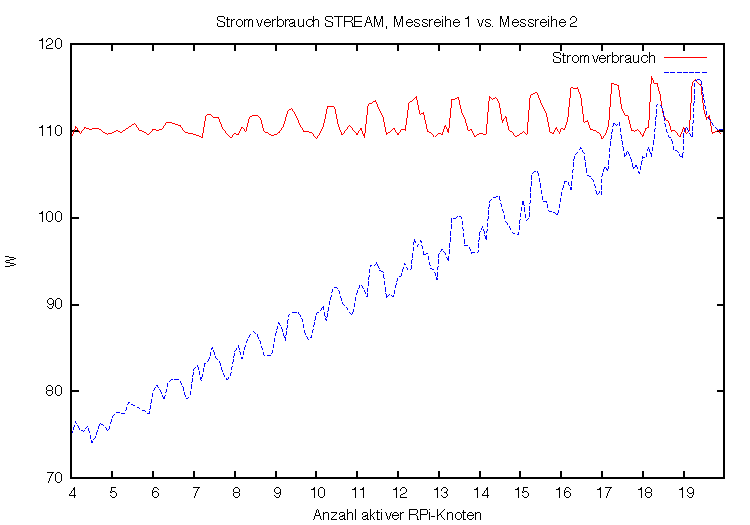
\includegraphics[scale=0.95]{strom5.pdf}\\ 
  \caption{Stromverbrauch f"ur STREAM, Messreihe 1 und Messreihe 2.}\label{fig:strom5}
\end{figure}
\endinput 


